\section{Führe die Katze}
In dieser Aufgabe bauen wir ein kleines Spiel. Es soll eine Katze auf einer Rennbahn gef{\"u}hrt werden ohne, dass die Wand ber{\"u}hrt werden darf. Einige von euch kennen ein {\"a}hnliches Spiel unter dem Namen \emph{hei{\ss}er Draht}.
\subsection{Male eine Rennbahn}
Wir brauchen eine Rennbahn für unsere Hauptfigur. Wir erzeugen dazu ein weiteres Sprite.
\begin{itemize}
\item[1. ] Klicke auf das \textit{Neues Objekt malen}-Icon
\end{itemize}
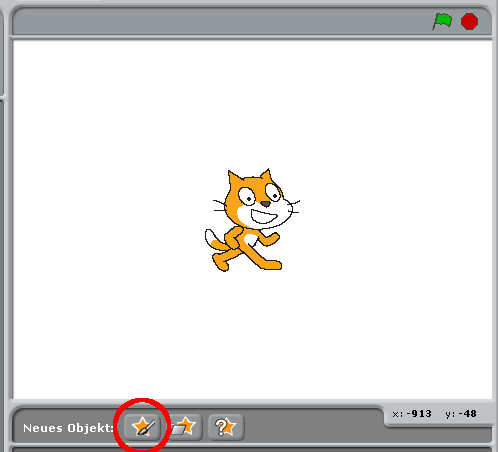
\includegraphics[width=0.6\textwidth]{images/aufgabe4_neues_objekt_malen.png}
\begin{itemize}
\item[2. ] Benutze das Zoom-Tool um komplett herauszuzoomen. Klicke auf die Minus-Lupe.
\end{itemize}
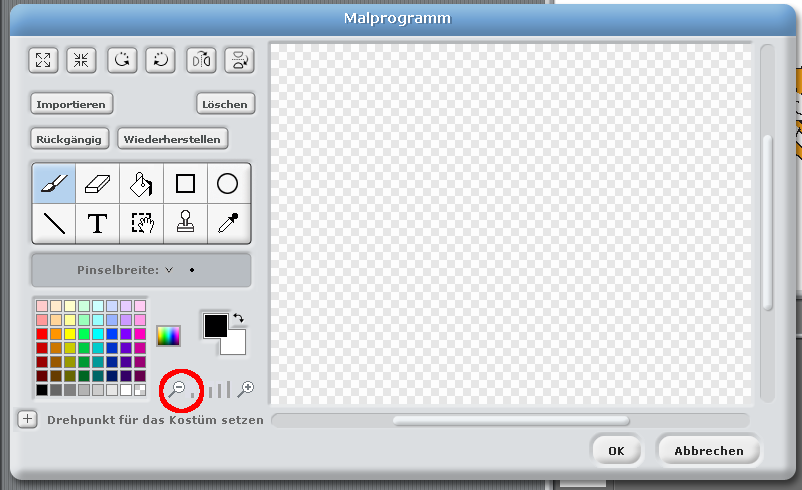
\includegraphics[width=0.6\textwidth]{images/aufgabe4_zoom.png}
\begin{itemize}
\item[3. ] Klicke auf den Pinsel um diesen auszuw{\"a}hlen, w{\"a}hle einen dickeren Pinsel und die Farbe grau.
\end{itemize}
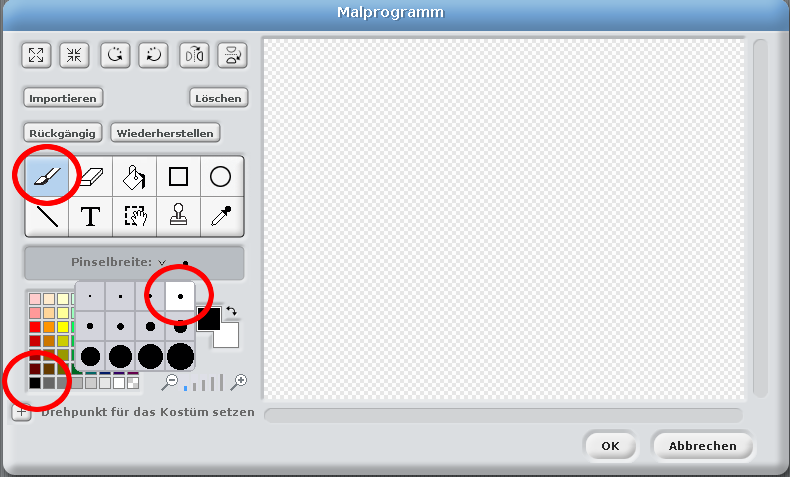
\includegraphics[width=0.6\textwidth]{images/aufgabe4_rennbahn_pinsel_waehlen.png}
\begin{itemize}
\item[4. ] Benutze den Pinsel um eine Rennbahn zu malen.
\end{itemize}
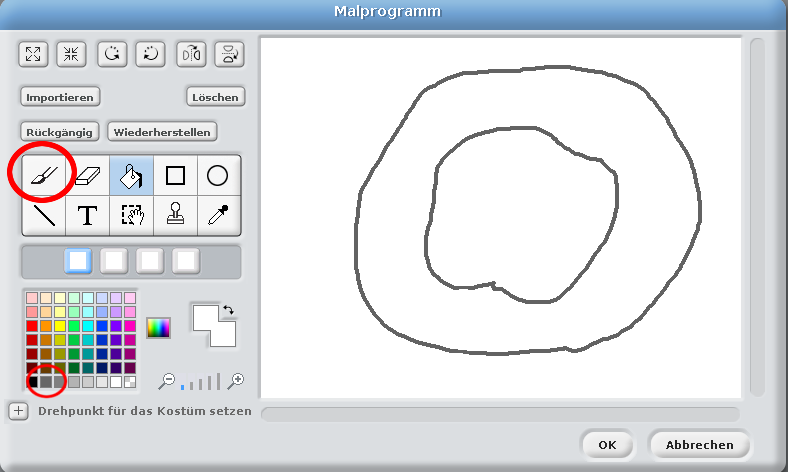
\includegraphics[width=0.6\textwidth]{images/aufgabe4_rennbahn_malen_00.png}
\begin{itemize}
\item[5. ] Da das jetzt einer Rennbahn noch nicht so {\"a}hnlich sieht f{\"u}llen wir die Rennfl{\"a}che mit der Farbe \emph{hellgr{\"u}n} und den Berg in der Mitte mit der Farbe \emph{braun} und alles andere Hellblau. Du kannst die Fl{\"a}chen mit dem Pinsel anmalen, leichter ist es jedoch mit dem \emph{Farbeimer}. Dazu einfach den Farbeimer und die Farbe ausw{\"a}hlen und dann auf die gew{\"u}nschte Fl{\"a}che klicken.
\end{itemize}
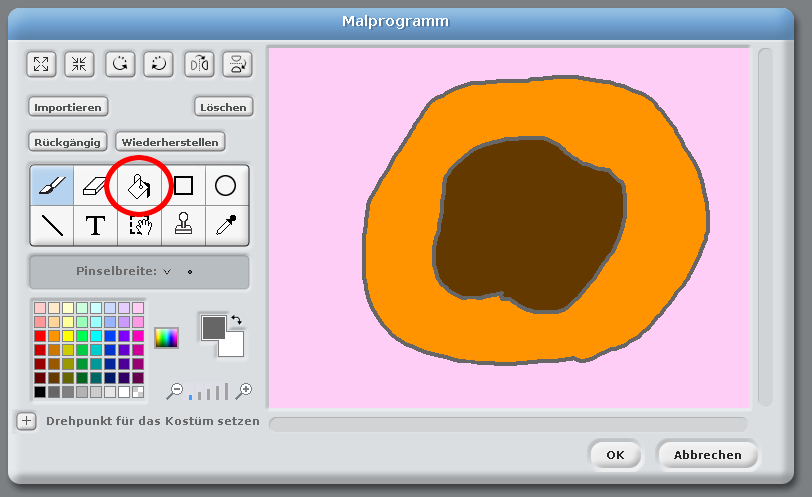
\includegraphics[width=0.6\textwidth]{images/aufgabe4_rennbahn_malen_01.png}
\begin{itemize}
\item[6. ] Zum Schluss f{\"u}gen wir noch ein weiteren Sprite hinzu und zwar eine \emph{Start/Ziel-Linie} in der Farbe \emph{rot}, diese erstellen und auf die gew{\"u}nschte Position schieben.
\end{itemize}
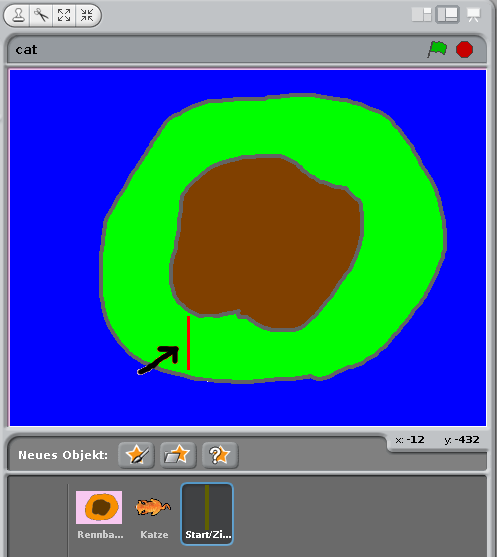
\includegraphics[width=0.6\textwidth]{images/aufgabe4_rennbahn_malen_02.png}
\begin{itemize}
\item[7.] Ändere den Namen des Sprites zu \textit{Rennbahn} und den Namen des Sprites f{\"u}r die Start/Ziel-Linie zu \textit{Start/Ziel}.
\end{itemize}

\subsection{Katze einf{\"u}gen}

\begin{itemize}
\item[1.] F{\"u}ge den Sprite \emph{Katze} aus einer Datei hinzu.
\end{itemize}
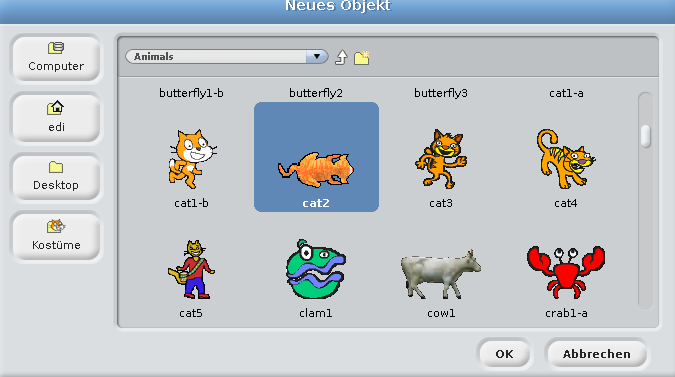
\includegraphics[width=0.6\textwidth]{images/aufgabe4_katze_sprite.png}
\begin{itemize}
\item[2. ] Ändere den Namen des Sprites zu Katze.
\end{itemize}
\begin{itemize}
\item[3.] Benutze das Verkleinerungs-Tool, um die Größe deiner Katze soweit zu verkleinern, dass sie zur Größe der Bahn passt und ohne anzusto{\ss}en auf der Bahn laufen kann.
\end{itemize}
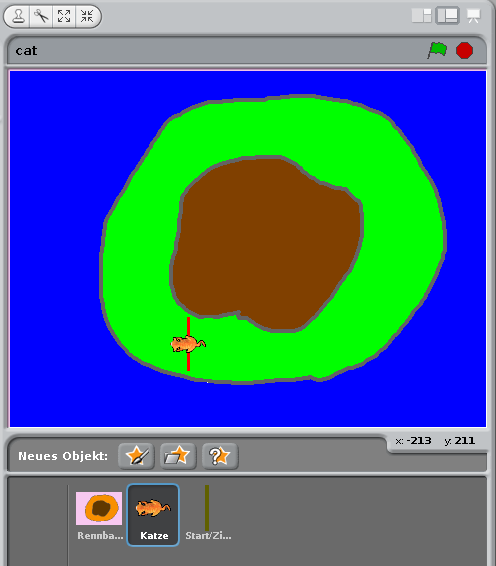
\includegraphics[width=0.6\textwidth]{images/aufgabe4_katze_schrumpfen.png}

\subsection{Erzeuge das Script für die Steuerung der Katze}

\begin{itemize}
\item[1. ] Klicke auf den Sprite Katze.
\item[2. ] Ziehe folgende Kacheln in dein Skript-Panel:
  \begin{itemize}
  \item[1. ] Aus dem Steuerungs-Panel die Kachel \textit{Wenn Taste Leertaste gedr{\"u}ckt} und \textit{falls...sonst} und setze beide zusammen.
  \item[2. ] Aus dem F{\"u}hlen-Panel die Kachel \textit{wird Farbe ber{\"u}hrt}. Diese Kachel setzt du als Bedingung in die \textit{falls...sonst}-Kachel
  \item[3. ] Aus dem AussehensPanel suchst du die Kachel \textit{sage Hallo! f{\"u}r 2 Sek.} raus und f{\"u}gst diese in den Bereich \textit{falls}, der \textit{falls...sonst}-Kachel ein.
  \item[4. ] Im Bewegungs-Panel findest du nun die vier letzten Kacheln f{\"u}r die Steuerung der Katze: \textit{zeige in Richtung 90} und \textit{gehe zu} f{\"u}gst du in den \textit{falls}-Bereich, gleich nach der Kachel \textit{sage Hallo! f{\"u}r 2 Sek.} ein. In den \textit{sonst}-Bereich ziehst du die beiden Kacheln \textit{zeige in Richtung 90} und \textit{gehe 10-er Schritt}.
  \end{itemize}
\end{itemize}
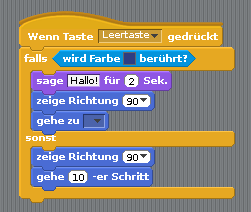
\includegraphics[width=0.6\textwidth]{images/aufgabe4_katze_bewegung_default.png}
\begin{itemize}
\item[3. ] Bei der Kachel \textit{Wenn Tast Leertaste gedr{\"u}ckt} klickst du auf den Text \textit{Leertaste} und w{\"a}hlst aus der Liste \textit{Pfeil nach oben}.
\item[4. ] Bei der Kachel \textit{wird Farbe ber{\"u}hrt} auf die Farbe klicken und dann auf den grauen Rand unserer Rennbahn.
\item[5. ] Bei der Kachel \textit{sage Hallo! f{\"u}r 2 Sek.} auf den Text \textit{Hallo!} klicken und diesen zu \textit{Au!} {\"a}ndern.
\item[6. ] Bei der Kachel \textit{zeige in Richtung 90} im \textit{falls}-Bereich auf die Zahl \textit{90} klicken und aus der Liste \textit{(-90) links} ausw{\"a}hlen.
\item[7. ] Bei der Kachel \textit{gehe zu} auf den kleinen Pfeil klicken und unseren Sprite \textit{Start/Ziel} aus der Liste ausw\"ahlen.
\item[7. ] Bei der Kachel \textit{zeige in Richtung 90} im \textit{sonst}-Bereich auf die Zahl \textit{90} klicken und aus der Liste \textit{(0) oben} ausw{\"a}hlen.
\item[8. ] Bei der letzten Kachel \textit{gehe 10-er Schritt} soll die Zahl \textit{10} durch eine \textit{2} ersetzt werden.
\end{itemize}
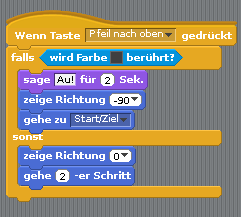
\includegraphics[width=0.6\textwidth]{images/aufgabe4_bewege_katze_nach_oben.png}

\begin{itemize}
\item[9. ] Das Ganze jeweils f{\"u}r die drei restlichen Richtungen \textit{rechts}, \textit{unten} und \textit{links} wiederholen und dabei nicht vergessen bei der Kachel \textit{zeige in Richtung 90} jeweils die gew{\"u}nschte Richtung ausw{\"a}hlen und die richtige Taste zu \"andern.
\end{itemize}

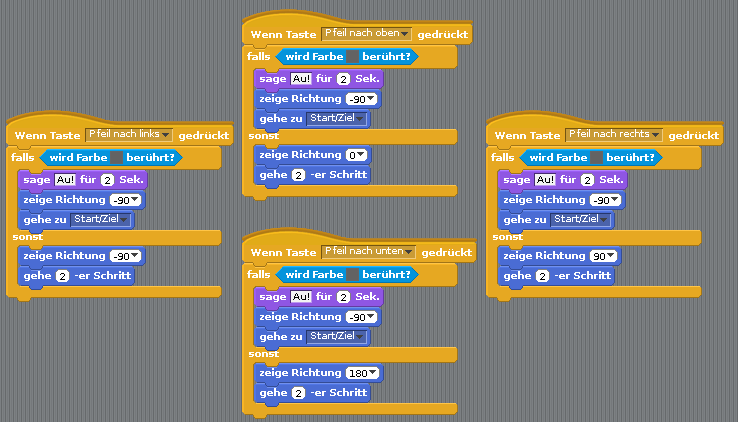
\includegraphics[width=0.6\textwidth]{images/aufgabe4_katze_alle_richtungen.png}
\begin{itemize}
\item[10. ] Um die Katze beim Start des Spiels zur Startlinie zu bringen, f{\"u}ge die Kacheln \textit{Wenn Fahne angeklickt} aus dem Steuerungs-Panel, aus dem Bewegungs-Panel \textit{zeige Richtung 90} und \textit{gehe zu} ein und setze diese zusammen.
\item[11. ] Bei der Kachel \textit{zeige in Richtung 90} im \textit{sonst}-Bereich auf die Zahl \textit{90} klicken und aus der Liste \textit{(-90) links} ausw{\"a}hlen.
\item[12. ] Bei der Kachel \textit{gehe zu} auf den Pfeil klicken und aus dem Men{\"u} und \textit{Start/Ziel} ausw{\"a}hlen.
\end{itemize}
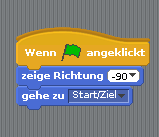
\includegraphics[width=0.6\textwidth]{images/aufgabe4_katze_an_start_stop.png}

\subsection{Zusatzaufgabe: Erweitere das Spiel damit zwei Spieler spielen k{\"o}nnen}
Du kannst einen weiteren Sprite hinzuf\"ugen und dir weitere vier Tasten auf der Tastatur aussuchen um diesen auch eine Steuerung zu geben. Hier die kurze Beschreibung wie man das machen k\"onnte:
\begin{itemize}
\item[1. ] Die vier Tasten f\"ur die Steuerung \"uberlegen z.B.
  \begin{itemize}
  \item w = oben
  \item d = rechts
  \item s = unten
  \item a = links
\end{itemize}
\item[2. ] Kopiere die Katze und passe die Skripte an, sodass die von dir ausgew\"ahlten Tasten zur Steuerung der Katze benutzt werden]
  \item[3. ] \"Andere das Aussehen einer Katze um es leichter zu machen sie zu Unterscheiden (wir haben ihr ein paar Punkte gegeben).
\end{itemize}
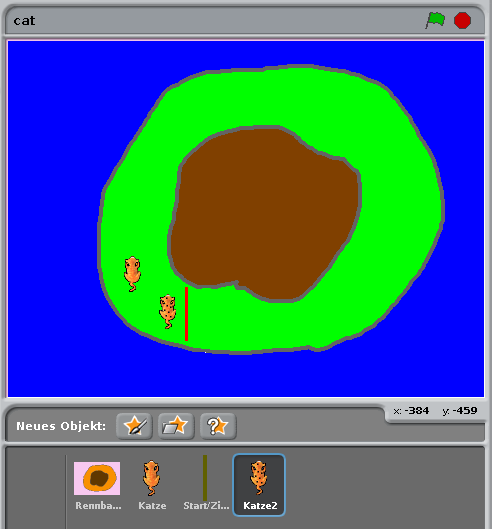
\includegraphics[width=0.6\textwidth]{images/aufgabe4_multiplayer.png}
